\documentclass[tikz,border=10pt]{standalone}
\usepackage{amsmath,amssymb}
\usepackage{tikz}
\usetikzlibrary{arrows,automata,backgrounds,calendar,chains,decorations,decorations.pathreplacing,decorations.text,fit,matrix,mindmap,patterns,petri,plotmarks,positioning,shadows,shapes,shapes.callouts,shapes.geometric,shapes.misc,spy,trees,calc,intersections,tikzmark,arrows.meta}
\usepackage{xcolor}
\usepackage{pgfplots}
\pgfplotsset{compat=1.16}

% Common math macros from the book
\def\x{\mathbf{x}}
\def\y{\mathbf{y}}
\def\z{\mathbf{z}}
\def\A{\mathbf{A}}
\def\b{\mathbf{b}}
\def\c{\mathbf{c}}
\def\w{\mathbf{w}}
\def\v{\mathbf{v}}
\def\u{\mathbf{u}}
\def\e{\mathbf{e}}
\def\zero{\mathbf{0}}
\def\R{\mathbb{R}}
\def\N{\mathbb{N}}
\def\Z{\mathbb{Z}}
\def\Q{\mathbb{Q}}
\def\st{\text{s.t.}}
\def\vect#1{\mathbf{#1}}
\def\xLP{x^{\mathrm{LP}}}
\def\zLP{z^{\mathrm{LP}}}
\def\xIP{x^{\mathrm{IP}}}

% Common node styles from the book
\tikzset{
    main/.style={circle, draw, fill=gray!20, minimum size=1cm, font=\normalsize},
    dot/.style={circle,fill=blue,minimum size=3pt,inner sep=0pt, outer sep=-1pt},
    vertex/.style={circle,fill=black!25,minimum size=20pt,inner sep=0pt},
    edge/.style={draw,-,thick},
    directed edge/.style={draw,->,>=latex,thick},
}

% Additional macros for 3D/coordinate systems
\newcommand{\xhat}{\hat{\x}}
\newcommand{\yhat}{\hat{\y}}
\newcommand{\zhat}{\hat{\z}}
\newcommand{\ihat}{\hat{\imath}}
\newcommand{\jhat}{\hat{\jmath}}
\newcommand{\khat}{\hat{k}}

\begin{document}
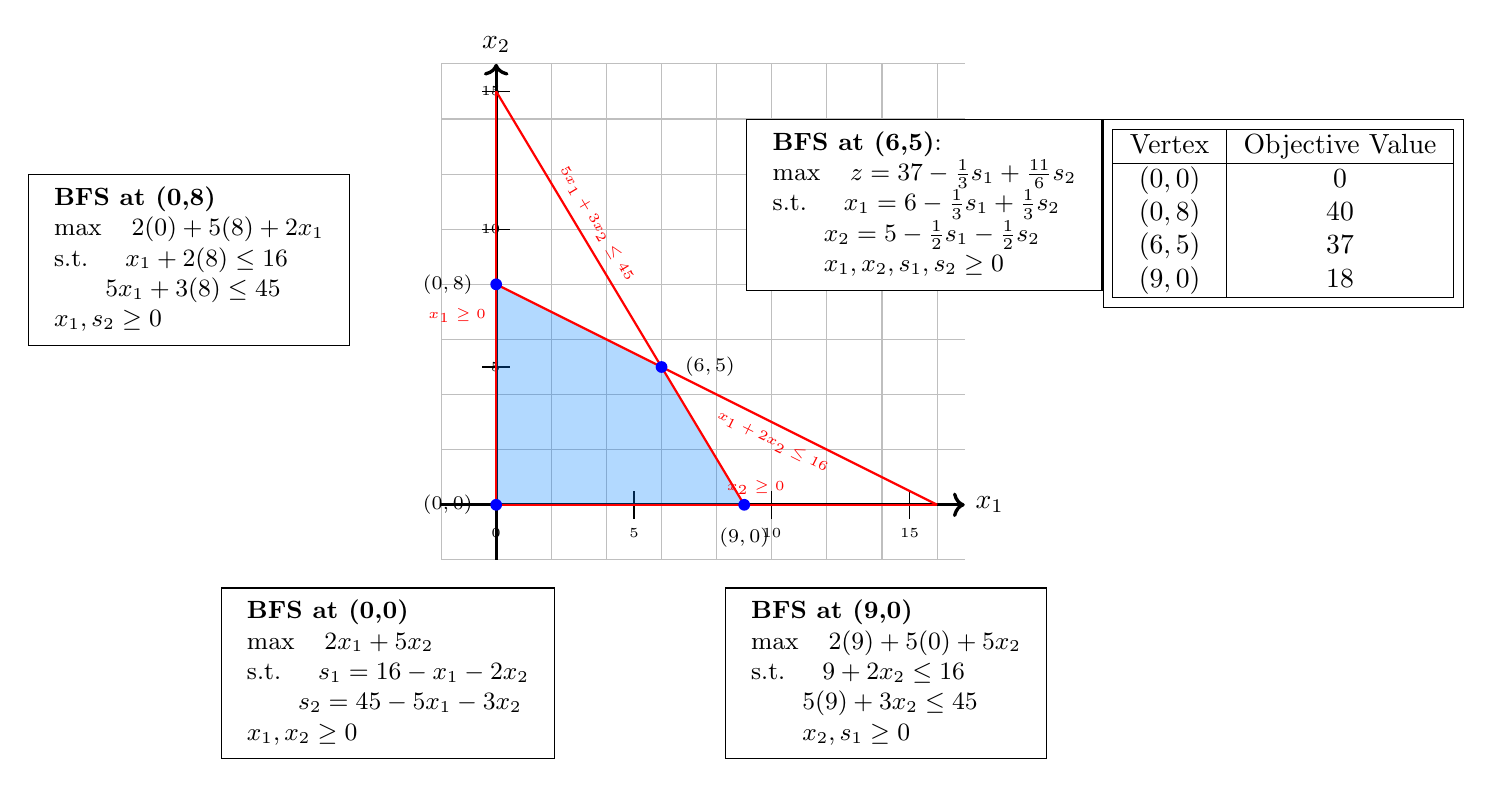
\begin{tikzpicture}[scale = 0.35]
    % Grid and axes
    \draw[gray!50, thin, step=2] (-2,-2) grid (17,16);
    \draw[very thick,->] (-2,0) -- (17,0) node[right] {$x_1$};
    \draw[very thick,->] (0,-2) -- (0,16) node[above] {$x_2$};

    % Axis labels
    \foreach \x in {0,5,10,15} \draw (\x,0.5) -- (\x,-0.5) node[below] {\tiny\x};
    \foreach \y in {0,5,10,15} \draw (-0.5,\y) -- (0.5,\y) node[left] {\tiny\y};

    % Shaded feasible region
    \fill[blue!50!cyan,opacity=0.3] (0,0) -- (0,8) -- (6,5) -- (9,0) -- cycle;

    % Constraint lines
    \draw[red,thick] (0,8) -- node[below right,sloped] {\tiny$x_1 + 2x_2 \leq 16$} (16,0);
    \draw[red,thick] (0,15) -- node[above left,sloped] {\tiny$5x_1 + 3x_2 \leq 45$} (9,0);
    \draw[red,thick] (0,0) -- node[below left] {\tiny$x_1 \geq 0$} (0,15);
    \draw[red,thick] (0,0) -- node[above right] {\tiny$x_2 \geq 0$} (16,0);

    % Vertices
    \node[blue] at (0,0) [circle,fill,inner sep=1.5pt]{};
    \node[blue] at (0,8) [circle,fill,inner sep=1.5pt]{};
    \node[blue] at (6,5) [circle,fill,inner sep=1.5pt]{};
    \node[blue] at (9,0) [circle,fill,inner sep=1.5pt]{};

    % Labels for vertices
    \node[black,anchor=east] at (-0.5,0) {\scriptsize$(0,0)$};
    \node[black,anchor=east] at (-0.5,8) {\scriptsize$(0,8)$};
    \node[black,anchor=west] at (6.5,5) {\scriptsize$(6,5)$};
    \node[black,anchor=north] at (9,-0.5) {\scriptsize$(9,0)$};

    % Optimization problems at each BFS
    \node[draw,fill=white,anchor=north west] at (-10,-3) {
        \small \begin{tabular}{l}
        \textbf{BFS at (0,0)} \\
        \(\max \quad 2x_1 + 5x_2\) \\
        \(\text{s.t. } \quad s_1 = 16 - x_1 - 2x_2\) \\
        \(\quad \quad  s_2 = 45 - 5x_1 - 3x_2\) \\
        \( x_1, x_2 \geq 0 \)
        \end{tabular}
    };

    \node[draw,fill=white,anchor=north west] at (-17,12) {
        \small \begin{tabular}{l}
        \textbf{BFS at (0,8)} \\
        \(\max \quad 2(0) + 5(8) + 2x_1\) \\
        \(\text{s.t. } \quad x_1 + 2(8) \leq 16\) \\
        \(\quad \quad 5x_1 + 3(8) \leq 45\) \\
        \( x_1, s_2 \geq 0 \)
        \end{tabular}
    };

    \node[draw,fill=white,anchor=north east] at (22,14) {
        \small \begin{tabular}{l}
        \textbf{BFS at (6,5)}:\\
        \(\max \quad z = 37 - \frac{1}{3}s_1 + \frac{11}{6}s_2\) \\
        \(\text{s.t. } \quad x_1 = 6 - \frac{1}{3}s_1 + \frac{1}{3}s_2\) \\
        \quad\quad \(x_2 = 5 - \frac{1}{2}s_1 - \frac{1}{2}s_2\)\\
        \quad\quad \( x_1, x_2, s_1, s_2 \geq 0 \)
        \end{tabular}
    };

    \node[draw,fill=white,anchor=north east] at (20,-3) {
        \small \begin{tabular}{l}
        \textbf{BFS at (9,0)} \\
        \(\max \quad 2(9) + 5(0) + 5x_2\) \\
        \(\text{s.t. } \quad 9 + 2x_2 \leq 16\) \\
        \(\quad \quad 5(9) + 3x_2 \leq 45\) \\
      \quad \quad  \( x_2, s_1 \geq 0 \)
        \end{tabular}
    };

    % Table within the TikZ picture
    \node[draw,fill=white,anchor=north west] at (22,14) {
        \begin{tabular}{|c|c|}
        \hline
        Vertex & Objective Value \\
        \hline
        $(0,0)$ & $0$ \\
        $(0,8)$ & $40$ \\
        $(6,5)$ & $37$ \\
        $(9,0)$ & $18$ \\
        \hline
        \end{tabular}
    };

\end{tikzpicture}
\end{document}
